\chapter{Foutafhandeling}

\begin{summary}
Tijdens het uitvoeren van een programma kan en zal er vanalles foutgaan. De gebruiker van het programma geeft de datum in in een foutief formaat, een printer is offline, er is onvoldoende schrijfruimte vrij om een bestand weg te schrijven, het programma kreeg onvoldoende geheugen toegewezen,... Fouten die zich voordoen tijdens het uitvoeren van een programma, at runtime dus, verdelen we onder in errors en exceptions. Errors zijn de fouten die meestal veroorzaakt worden door het onderliggende besturingssysteem. Tijdens het verloop van het programma kunnen deze errors niet meer opgelost worden en het programma zal daarom be\"eindigd worden. Dit is niet het geval voor exceptions. Je kan je code op een defensieve manier schrijven en rekening houden met de mogelijke exceptions die kunnen optreden. ``Exception handling'' is het proces om deze exceptions op een correcte en liefst gebruiksvriendelijke manier af te handelen. Indien een fout niet correct wordt afgehandeld, zal het programma alsnog voortijdig afgebroken worden, maar met de juiste foutafhandeling kan de uitvoer van het programma gewoon verdergezet worden. 
 \end{summary}
 
\section{Compile-time vs runtime errors}

Een programmeur schrijft Java code in zijn editor of favoriete IDE. Vervolgens wordt de Java code gecompileerd tot bytecode. Deze bytecode wordt door de JVM (Java Virtual Machine) ge\"interpreteerd tot machinecode instructies die worden uitgevoerd door het computersysteem.

Wanneer dus een Java programma wordt opgestart, kunnen er 2 categorie\"en van problemen voorkomen. Het kan zijn dat het Java programma niet gecompileerd kan worden. In dat geval spreken we van een compile-time error. Indien het programma succesvol gecompileerd wordt, kan er zich tijdens het uitvoeren van de code een probleem voordoen, in dat geval spreken we van runtime errors of exceptions. 

\begin{figure}[H]
  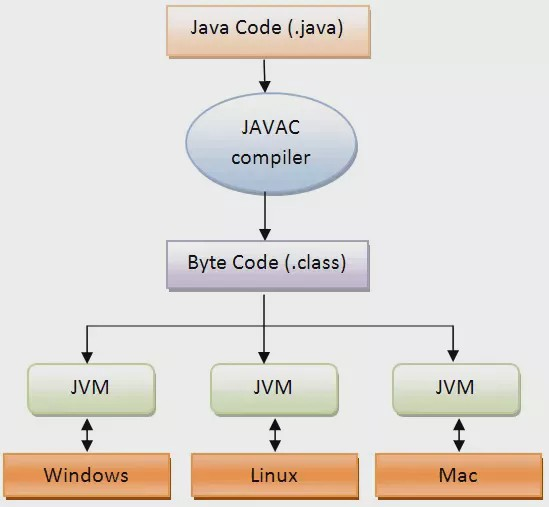
\includegraphics[width=\linewidth]{images/h1/java_compiler.jpeg}
  \caption{Compiler, interpreter en Java Virtual Machine.}
  \label{fig:compiler}
\end{figure}


\begin{figure}[H]
  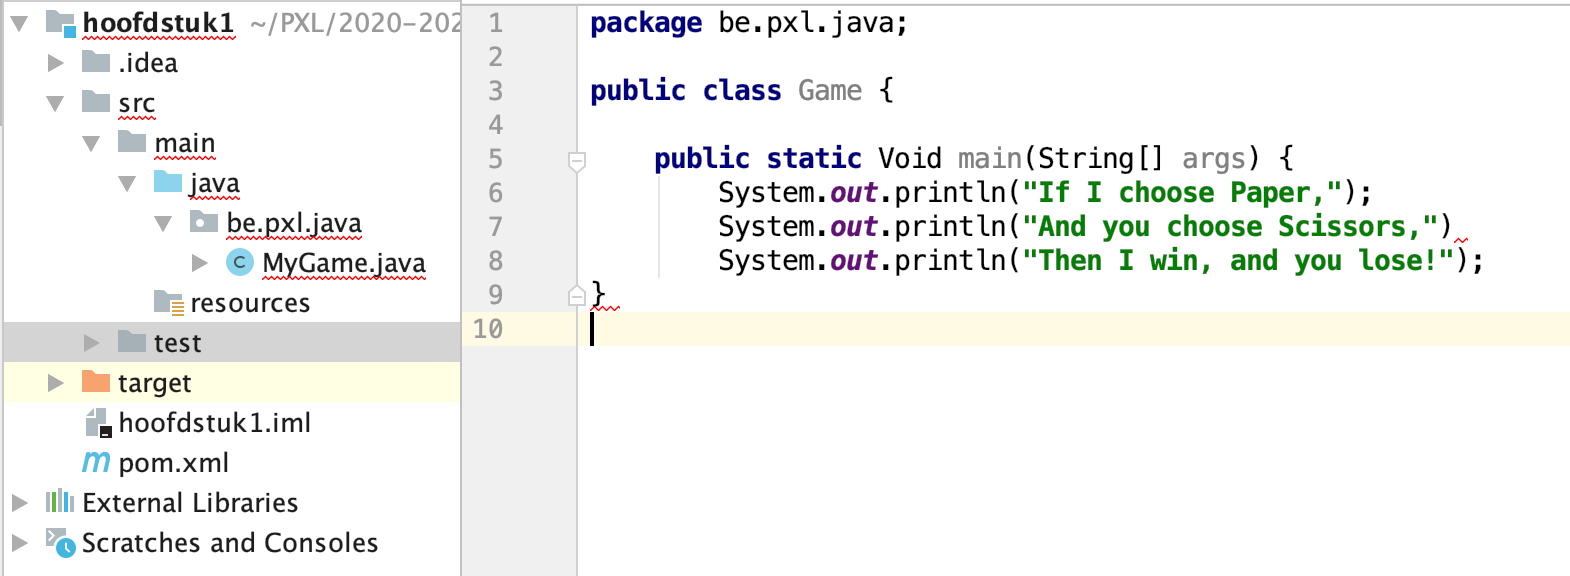
\includegraphics[width=\linewidth]{images/h1/compiletime_errors.png}
  \caption{Compile-time errors}
  \label{fig:compiletime_errors}
\end{figure}

\begin{oefening}
Welke compile-time errors kan je ontdekken in het volgende codefragment in figuur \ref{fig:compiletime_errors}?
\end{oefening}

Omdat Java een object-ge\"orienteerde programmeertaal is, wordt er ook een object gebruikt om aan te geven dat er iets fout ging bij uitvoeren van het Java programma. Zodra er zich een probleem voordoet tijdens het uitvoeren van een programma-instructie, wordt er een exception-object aangemaakt en ``opgeworpen''. Hierdoor stopt de normale uitvoer van het programma. Er wordt nog geprobeerd om het exception-object op een keurige manier af te handelen (indien die code aanwezig is), maar als dat niet lukt zal het programma be\"eindigd worden. Het exception-object bevat nuttige informatie voor de ontwikkelaar zoals de methode en lijn-nummer waar de exception werd aangemaakt en het type van de exception. 

\section{First catch}

\begin{lstlisting}
public class DivisionByZero {

	public static void main(String[] args) {
		int a = (1 + 1) % 2;
		int b = 5;
		int c = b / a;
		System.out.println("Het resultaat is " + c);
	}
}
\end{lstlisting}

Als je het bovenstaande programma uitvoert zal het volgende in de console verschijnen:

\begin{verbatim}
Exception in thread "main" java.lang.ArithmeticException: / by zero
	at be.pxl.ja.DivisionByZero.main(DivisionByZero.java:6)<5 internal calls>
\end{verbatim}
  
De variabele \textit{a} bevat inderdaad de waarde 0 en hierdoor hebben we dus te maken met een deling door 0. Zodra de deling wordt uitgevoerd loopt het dus fout en gooit de java runtime een ArithmeticException op. Omdat de ArithmeticException nergens wordt afgehandeld eindigt het programma. Je zal enkel nog een stacktrace zien verschijnen in de console. Een stacktrace is de naam en foutboodschap van de exception gevolgd door de weg die de exception heeft afgelegd (doorheen de methoden van je klassen) vanaf het moment dat ze werd opgegooid. We zien dus dat de exception is veroorzaakt op regel 6 in de klasse DivisionByZero.

\begin{lstlisting}
public class DivisionByZero {

	public static void main(String[] args) {
		int a = (1 + 1) % 2;
		int b = 5;
		try {
			int c = b / a;
			System.out.println("Het resultaat is " + c);
		} catch (ArithmeticException e) {
			System.out.println("You should not divide a number by zero.");
		}
		System.out.println("First catch completed!");
	}
}
\end{lstlisting}

\begin{verbatim}
You should not divide a number by zero.
First catch completed!
\end{verbatim}

We hebben de instructie met de deling nu in een try-blok geplaatst. Omdat de variabele c in het try-blok wordt aangemaakt, kan deze variabele ook enkel binnen het try-blok gebruikt worden. Indien een exception optreedt binnen een try-blok zal de programma-uitvoer de resterende code binnen het try-blok overslaan en verdergaan bij het eerste catch-blok dat direct volgt achter het try-blok. Je bent als programmeur verplicht om een try-blok steeds te laten volgen door \'e\'en of meerdere catch-blokken.
In het catch-blok wordt dan de code uitgevoerd om het probleem op te lossen of tenminste een duidelijke boodschap voor de gebruiker van het programma te voorzien.
Als alle instructies uit het catch-blok zijn uitgevoerd zal het programma zijn normale uitvoer verderzetten.


\section{Java exception hi\"erarchie}
  
\begin{figure}[H]
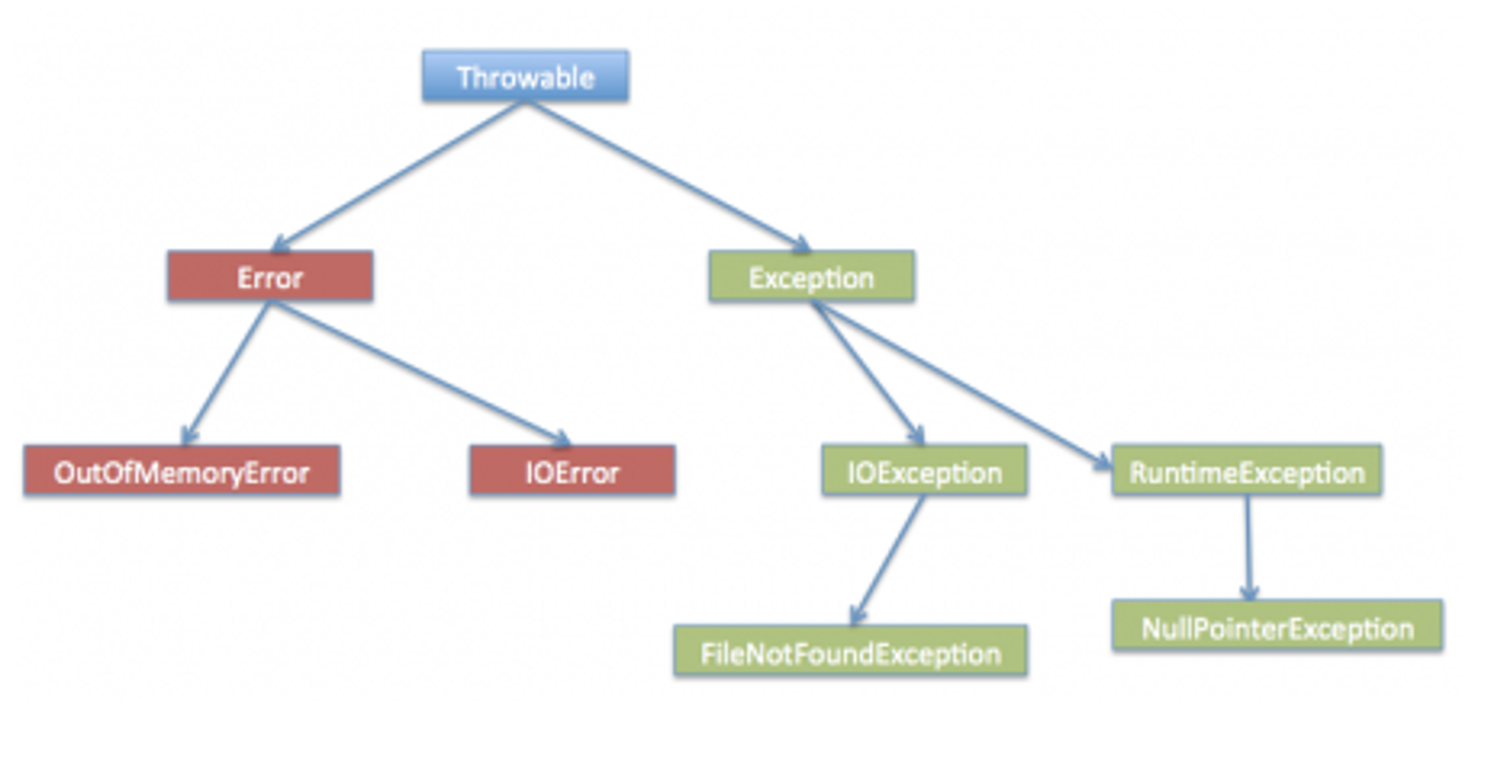
\includegraphics[width=\linewidth]{images/h1/exception-hierarchy.png}
\caption{Exception hi\"erarchie}
\label{fig:exceptiono_hierarchy}
\end{figure}
  
Zoals reeds vermeld wordt er een exception-object aangemaakt zodra zich een probleem voordoet in de code. 
Er is in Java een hi\"erarchie gebouwd van exception-klassen om verschillende soorten fouten in een programma te categorizeren. Throwable is de superklasse van alle exceptions en errors in Java. Er zijn dus 2 afgeleide klassen van Throwable: Error and Exception. Exceptions zijn nog verder onderverdeeld in \textbf{checked exceptions} en \textbf{runtime exceptions}.

\subsection{Errors}

Errors zijn problemen die zich voordoen tijdens het uitvoeren van het programma en die meestal niet gerelateerd zijn aan het programma zelf. Daarom is het onmogelijk om erop te anticiperen en te herstellen van deze fouten. Dit kan gaan van hardware falen, over JVM crashes en out of memory errors. We hebben een aparte hi\"erarchie van errors en we zullen nooit code toevoegen in ons programma om deze fouten af te handelen. We tonen hier enkel voorbeelden van errors.


\subsubsection{StackOverflowError}
Je hebt ongetwijfeld al eens per ongeluk een programma geschreven met een oneindige lus. 

\begin{lstlisting}
public class DemoStackOverflow {

	private static void printNumber(int x) {
		System.out.println(x);
		printNumber(x + 2);
	}

	public static void main(String[] args) {
		printNumber(15);
	}
}
\end{lstlisting}

\begin{verbatim}
15
17
19
...
36597
36599
Exception in thread "main" java.lang.StackOverflowError
	...
	at be.pxl.ja.DemoStackOverflow.printNumber(DemoStackOverflow.java:5)
	at be.pxl.ja.DemoStackOverflow.printNumber(DemoStackOverflow.java:5) 
	at be.pxl.ja.DemoStackOverflow.printNumber(DemoStackOverflow.java:5) 
	at be.pxl.ja.DemoStackOverflow.printNumber(DemoStackOverflow.java:5) 
	...
\end{verbatim}

De call stack is de manier waarop tijdens de uitvoer van een programma o.a. wordt bijgehouden welke functies worden aangeroepen. Wanneer je programma-uitvoer in een oneindige lus terechtkomt, stapelen de gegevens in de call stack zich razendsnel op en loopt de call stack vol. Het programma zal uiteindelijk eindigen met een StackOverflowError.

\begin{figure}[H]
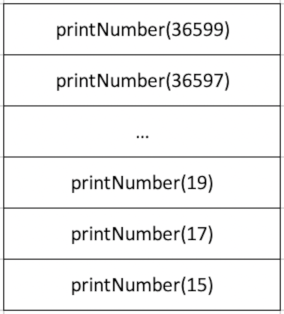
\includegraphics{images/h2/java_call_stack.png}
\caption{Java call stack}
\label{fig:call_stack}
\end{figure}


\subsubsection{OutOfMemoryError}

\begin{lstlisting}
public class DemoOutOfMemory {

	private void generateOutOfMemory() {
		Long maxMemory = Runtime.getRuntime().maxMemory();
		System.out.println(maxMemory);

		int[] matrix = new int[(int) (maxMemory + 1)];
		for (int i = 0; i < matrix.length; ++i) {
			matrix[i] = i + 1;
		}
		System.out.println("Matrix filled" + matrix[(int)(Math.random() * 100)]);

	}

	public static void main(String[] args) {
		DemoOutOfMemory doom = new DemoOutOfMemory();
		doom.generateOutOfMemory();
	}
}
\end{lstlisting}

Om de OutOfMemoryError te illustreren maken we een array aan die meer geheugenplaatsen inneemt dan de ruimte die het java programma ter beschikking heeft.

Als je dit programma uitvoert, pas je best het beschikbare geheugen voor het programma aan. Dit doe je door een waarde voor de VM optie -Xmx mee te geven.

\begin{itemize}
\item -Xmssize: Geeft de initi\"ele waarde voor de heap size.
\item -Xmxsize: Geeft de maximale waarde voor heap size.
\end{itemize}

De heap size van een Java programma is de hoeveelheid geheugen dat een Java-programma mag gebruiken om objecten op te slaan.

\begin{verbatim}
67108864
Exception in thread "main" java.lang.OutOfMemoryError: Java heap space
	at be.pxl.ja.DemoOutOfMemory.generateOutOfMemory(DemoOutOfMemory.java:8)
	at be.pxl.ja.DemoOutOfMemory.main(DemoOutOfMemory.java:16)<5 internal calls>
\end{verbatim}
	
\begin{figure}[H]
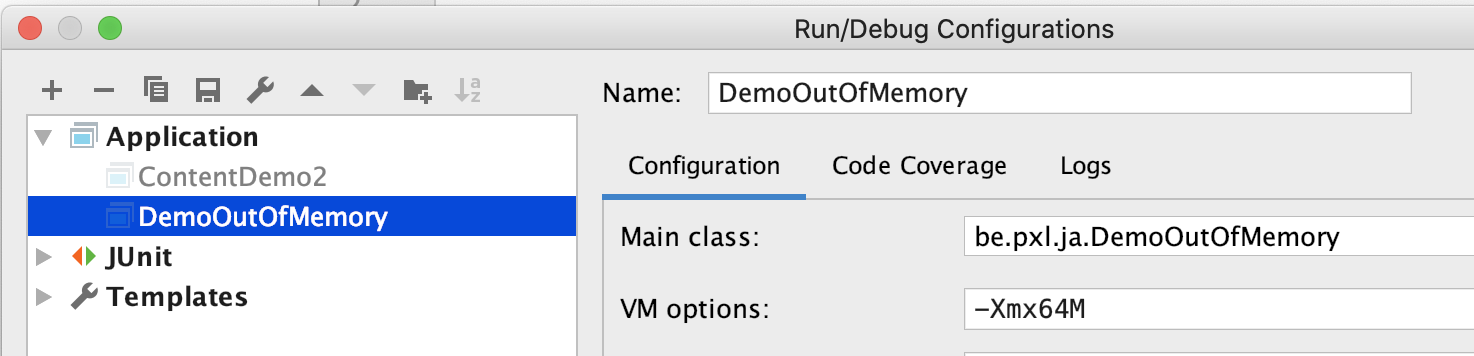
\includegraphics[width=\linewidth]{images/h2/jvm_options_xmx.png}
\caption{Maximum heap size aanpassen}
\label{fig:exceptiono_hierarchy}
\end{figure}

\subsection{Runtime exceptions}

Runtime exceptions zijn exceptions die vaak veroorzaakt worden door logische fouten in het programma.Typische voorbeelden van runtime exceptions zijn ArrayIndexOutOfBoundsException, NullPointerException en IllegalArgumentException. Vaak moet je ze niet afhandelen, maar moet je ervoor zorgen dat je de bug in je code oplost. Ook hier zijn onze unit testen heel belangrijk. Door goede unit testen te schrijven ga je runtime exceptions in je code opmerken en kunnen oplossen.

\begin{lstlisting}
public class Demo {

	public static void main(String[] args) {
		String tekst = "abc";
		System.out.println(tekst.repeat(-5));
	}
}
\end{lstlisting}

\begin{verbatim}
Exception in thread "main" java.lang.IllegalArgumentException: count is negative: -5
	at java.base/java.lang.String.repeat(String.java:3586)
	at be.pxl.ja.streamingservice.Demo.main(Demo.java:5)
\end{verbatim}

\begin{oefening}

\begin{lstlisting}
public class StreamingService {

	private List<Account> accounts;

	public void addAccount(Account account) {
		accounts.add(account);
	}
}
\end{lstlisting}

Welke exception doet zich voor zodra je voor een object van de klasse StreamingService de methode addAccount() aanroept? Waarom treedt die exception op?
\end{oefening}

Wanneer je programma gebruikmaakt van gegevens die door de gebruiker worden ingevoerd, moet je er altijd rekening mee houden dat de gebruiker foutieve gegevens kan ingeven. Deze foutieve gegevens kunnen aanleiding geven tot runtime exceptions. Ook hier moet je steeds anticiperen op de mogelijke input die de gebruiker kan invoeren. 


\begin{lstlisting}
public class ElementInArray {

	public static void main(String[] args) {
		String[] elements = { "H", "He", "Li", "Be", "B", "C", "N", "O", "F", "Ne" };

		Scanner scanner = new Scanner(System.in);
		
		// OPLOSSING 1
		System.out.println("Kies een nummer: ");
		int chosen = scanner.nextInt();
		if (chosen < elements.length) {
			System.out.println(elements[chosen]);
		} else {
			System.out.println("U koos een verkeerd nummer.");
		}

	    // OPLOSSING 2
		System.out.println("Kies een nummer: ");
		chosen = scanner.nextInt();
		try {
			System.out.println(elements[chosen]);
		} catch (ArrayIndexOutOfBoundsException e) {
			System.out.println("U koos een verkeerd nummer.");
		}
	}
}
\end{lstlisting}

In bovenstaand codevoorbeeld gaat onze voorkeur uit naar oplossing 1 waarbij de ingevoerde waarde wordt gecontroleerd vooraleer het element uit de array wordt benaderd. Deze code is makkelijker leesbaar en onderhoudbaar.

\begin{oefening}
Maak een programma dat de geboortedatum vraagt als input. Vervolgens berekent het programma hoeveel dagen het nog duurt vooraleer je jarig bent. Gebruik de methode parse() uit de klasse LocalDateTime om van de input van de gebruiker een LocalDateTime-object te maken. Welke exception kan optreden? Blijf input vragen totdat de gebruiker een correcte datum heeft ingegeven.
\end{oefening}


\subsection{Checked exceptions}

Wanneer je in java een methode aanroept, kan het voorkomen dat je direct een compileerfout voorgeschoteld krijgt. Het kan namelijk zijn dat java reeds anticipeert op mogelijke problemen en je dwingt om rekening te houden met het scenario dat er iets mis kan gaan. De compileerfout raakt pas opgelost wanneer je het afhandelen van de exception netjes programmeert.

Kijk eens naar onderstaand voorbeeld uit de streaming service.
We gebruiken hier de klasse MessageDigest uit JDK. Message digests zijn functies waarmee we voor input-data van willekeurige lengte een hash-waarde met een vaste lengte kunnen berekenen.  Als je de hash-waarde kent, kan je hieruit de input-data niet afleiden. We gebruiken dit om een paswoord bij te houden in een Account-object. We willen absoluut vermijden dat paswoorden in een leesbaar formaat in onze objecten worden bijgehouden.

Om een message digest te berekenen in Java moet je eerst de static methode getInstance() aanroepen met als parameter het door jouw gekozen algoritme. In dit voorbeeld wordt er gekozen voor MD5. Je ziet dat de lijn code, ondanks het feit dat alles correct is geschreven, toch rood wordt onderlijnd. Dat komt omdat de methode getInstance() een exception kan opgooien die we verplicht moeten afhandelen.

\begin{oefening}
Open de documentatie van de klasse MessageDigest en bekijk de uitleg voor de static methode getInstance(). Kan je hier zien welke exceptions er kunnen voorkomen?
\end{oefening}

\begin{figure}[H]
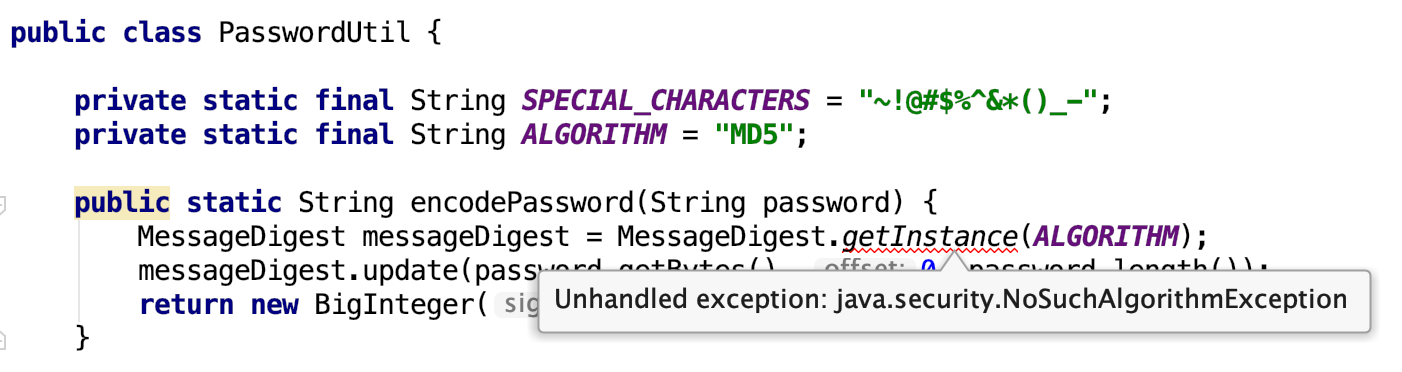
\includegraphics[width=\linewidth]{images/h2/no_such_algorithm_exception.png}
\caption{Een checked exception: NoSuchAlgorithmException}
\label{fig:no_such_algorithm}
\end{figure}

Deze compileerfout wordt veroorzaakt omdat de exception-klasse NoSuchAlgorithmException een checked exception is. Dit betekent dat het aanroepen van de methode die de exception gooit een compileerfout zal geven, omdat er geen code is toegevoegd om correct met de  exception om te gaan.
Er zijn 2 mogelijke oplossingen om deze compileerfout aan te pakken. Ofwel vang de exception op en handel je ze af in de methode encodePassword(), ofwel voeg je in de signatuur van de methode encodePassword() toe dat je de methode toelaat om een NoSuchAlgorithmException op te werpen. We geven nu eerst een voorbeeld van hoe je de exception kan opvangen en afhandelen. 

\begin{lstlisting}
import be.pxl.ja.streamingservice.util.PasswordUtil;

public class Account {
	private String email;
	private String password;

	public Account(String email, String password) {
		this.email = email;
		setPassword(password);
	}

	public String getEmail() {
		return email;
	}

	public void setEmail(String email) {
		this.email = email;
	}

	public boolean verifyPassword(String password) {
		return PasswordUtil.isValid(password, this.password);
	}

	public void setPassword(String password) {
		this.password = PasswordUtil.encodePassword(password);
	}
}
\end{lstlisting}

\begin{lstlisting}
import java.math.BigInteger;
import java.security.MessageDigest;
import java.security.NoSuchAlgorithmException;

public class PasswordUtil {

	private static final String ALGORITHM = "MD5";

	public static String encodePassword(String password) {
		MessageDigest messageDigest = null;
		try {
			messageDigest = MessageDigest.getInstance(ALGORITHM);
		} catch (NoSuchAlgorithmException e) {
			return null;
		}
		messageDigest.update(password.getBytes(), 0, password.length());
		return new BigInteger(1, messageDigest.digest()).toString(16);
	}

	public static boolean isValid(String providedPassword, String securedPassword) {
		return encodePassword(providedPassword).equals(securedPassword);
	}
}
\end{lstlisting}


\begin{lstlisting}
import be.pxl.ja.streamingservice.model.Account;

public class CheckedExceptionDemo {

	public static void main(String[] args) {
		Account newAccount = new Account("daffy@duckstad.be", "daffy123!");
		System.out.println(newAccount.verifyPassword("daffy123"));
		System.out.println(newAccount.verifyPassword("daffy123!"));
	}
}
\end{lstlisting}

Het algoritme ``MD5'' is een geldige waarde voor de parameter algorithm en je krijgt een probleemloos verloop van je programma. Maar een programmeur die zich vergist en de constante ALGORITHM in de klasse PasswordUtil de waarde ``MD4'' geeft zal een probleem veroorzaken.

\begin{verbatim}
Exception in thread "main" java.lang.NullPointerException
	at be.pxl.ja.streamingservice.util.PasswordUtil.isValid(PasswordUtil.java:24)
	at be.pxl.ja.streamingservice.model.Account.verifyPassword(Account.java:37)
	at be.pxl.ja.streamingservice.CheckedExceptionDemo.main(CheckedExceptionDemo.java:9)
\end{verbatim}

\begin{figure}[H]
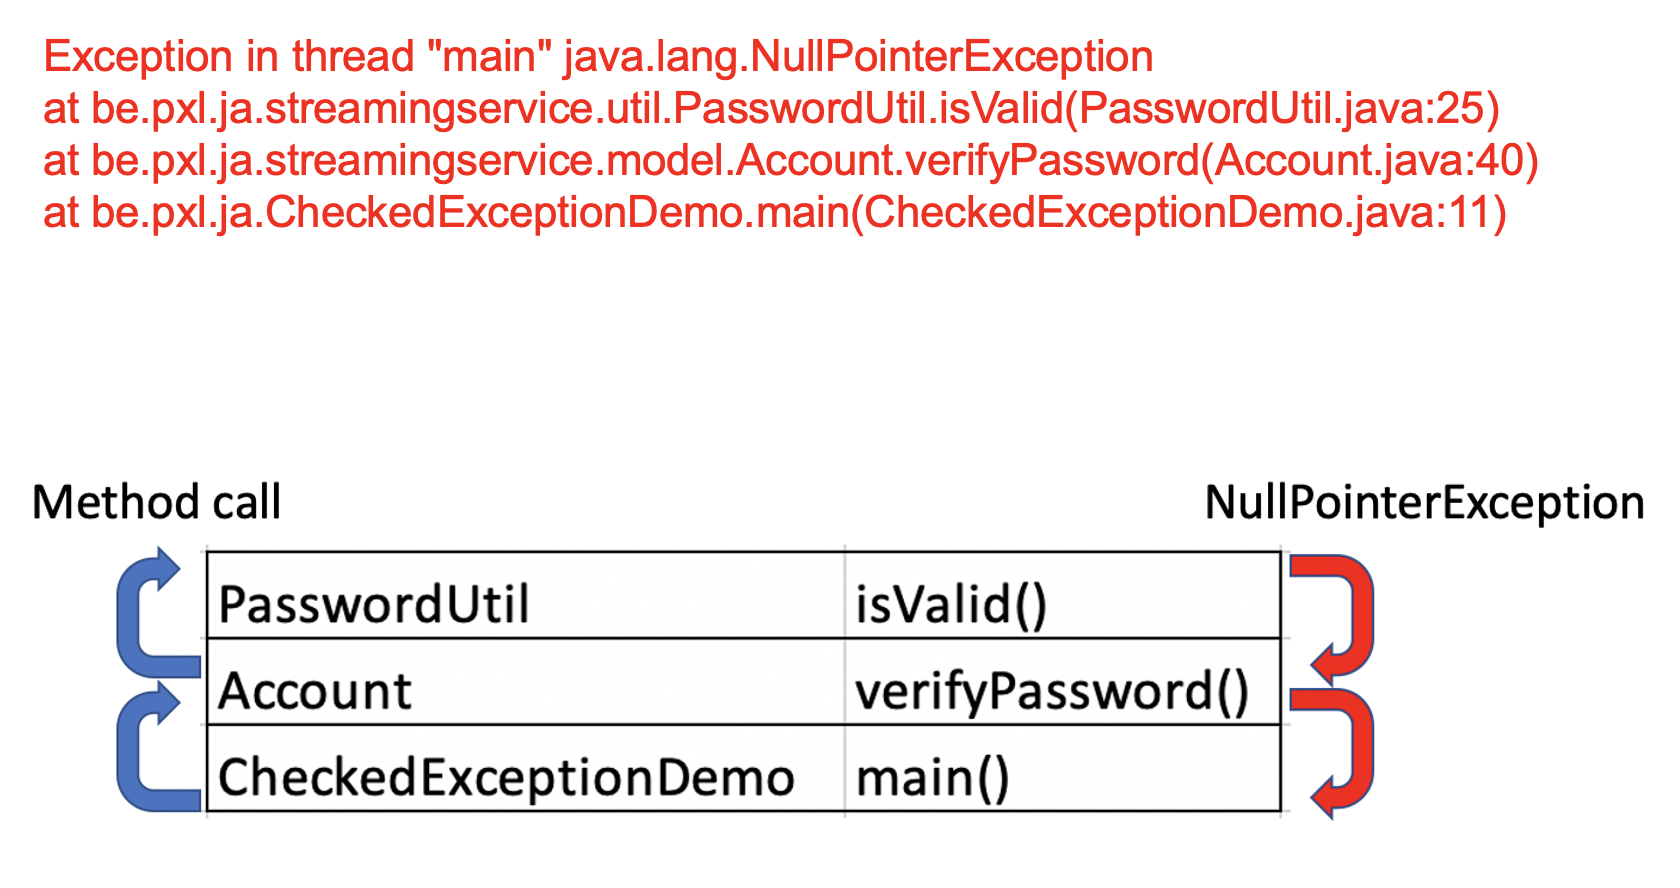
\includegraphics[width=\linewidth]{images/h2/exception_call_stack.png}
\caption{Method call stack}
\label{fig:method_call_stack}
\end{figure}

De NoSuchAlgorithmException wordt afgehandeld door null te geven als returnwaarde van de methode encodePassword.  Hierdoor wordt het probleem pas opgemerkt op het ogenblik dat we de methode isValid van de klasse PasswordUtil gebruiken. De informatie dat het foute algoritme werd meegegeven is momenteel volledig verloren gegaan. Daarom wordt altijd aangeraden om exceptions die zich voordoen in je programma bij te houden in logbestanden. Het gebruik van logbestanden valt buiten de scope van deze cursus. Als alternatief voor het loggen van exceptions zullen we in deze cursus de stacktrace van de exception tonen in de console.

\begin{lstlisting}
import java.math.BigInteger;
import java.security.MessageDigest;
import java.security.NoSuchAlgorithmException;

public class PasswordUtil {

	private static final String ALGORITHM = "MD4";

	public static String encodePassword(String password) {
		MessageDigest messageDigest = null;
		try {
			messageDigest = MessageDigest.getInstance(ALGORITHM);
		} catch (NoSuchAlgorithmException e) {
			e.printStackTrace();
			return null;
		}
		messageDigest.update(password.getBytes(), 0, password.length());
		return new BigInteger(1, messageDigest.digest()).toString(16);
	}

	public static boolean isValid(String providedPassword, String securedPassword) {
		return encodePassword(providedPassword).equals(securedPassword);
	}
}
\end{lstlisting}
 
Door de stacktrace te tonen in de console raken we geen cruciale informatie kwijt.

\begin{verbatim}
java.security.NoSuchAlgorithmException: MD4 MessageDigest not available
	at java.base/sun.security.jca.GetInstance.getInstance(GetInstance.java:159)
	at java.base/java.security.Security.getImpl(Security.java:700)
	at java.base/java.security.MessageDigest.getInstance(MessageDigest.java:177)
	at be.pxl.ja.streamingservice.util.PasswordUtil.encodePassword(PasswordUtil.java:15)
	at be.pxl.ja.streamingservice.model.Account.setPassword(Account.java:45)
	at be.pxl.ja.streamingservice.model.Account.<init>(Account.java:16)
	at be.pxl.ja.streamingservice.CheckedExceptionDemo.main(CheckedExceptionDemo.java:8)
java.security.NoSuchAlgorithmException: md4 MessageDigest not available
	at java.base/sun.security.jca.GetInstance.getInstance(GetInstance.java:159)
	at java.base/java.security.Security.getImpl(Security.java:700)
	at java.base/java.security.MessageDigest.getInstance(MessageDigest.java:177)
	at be.pxl.ja.streamingservice.util.PasswordUtil.encodePassword(PasswordUtil.java:15)
	at be.pxl.ja.streamingservice.util.PasswordUtil.isValid(PasswordUtil.java:25)
	at be.pxl.ja.streamingservice.model.Account.verifyPassword(Account.java:37)
	at be.pxl.ja.streamingservice.CheckedExceptionDemo.main(CheckedExceptionDemo.java:9)
Exception in thread "main" java.lang.NullPointerException
	at be.pxl.ja.streamingservice.util.PasswordUtil.isValid(PasswordUtil.java:25)
	at be.pxl.ja.streamingservice.model.Account.verifyPassword(Account.java:37)
	at be.pxl.ja.streamingservice.CheckedExceptionDemo.main(CheckedExceptionDemo.java:9)
\end{verbatim}

Opnieuw zie je het belang van unit testen. Een foute waarde voor het gekozen algoritme ga je al heel snel opmerken en herstellen als je unit testen schrijft voor de methoden encodePassword() en isValid().

In dit voorbeeld is het eigenlijk aangewezen om de exception niet af te handelen. Een alternatief is dat we de methode encodePassword() toelaten om de exception, als die zich voordoet, gewoon verder door te geven (gooien).
Hierdoor komt de exception dus terecht op de plaatsen waar je de methode encodePassword() gaat aanroepen en moet je op die plaatsen afhandeling voorzien. Je kan er dus voor kiezen om de checked exception NoSuchAlgorithmException helemaal mee te sleuren doorheen je applicatie tot aan de main()-methode.

\begin{lstlisting}
import java.math.BigInteger;
import java.security.MessageDigest;
import java.security.NoSuchAlgorithmException;

public class PasswordUtil {

	private static final String ALGORITHM = "MD5";

	public static String encodePassword(String password) throws NoSuchAlgorithmException {
		MessageDigest messageDigest = MessageDigest.getInstance(ALGORITHM);
		messageDigest.update(password.getBytes(), 0, password.length());
		return new BigInteger(1, messageDigest.digest()).toString(16);
	}

	public static boolean isValid(String providedPassword, String securedPassword) throws NoSuchAlgorithmException {
		return encodePassword(providedPassword).equals(securedPassword);
	}
}
\end{lstlisting}

\begin{lstlisting}
import java.security.NoSuchAlgorithmException;
import java.util.ArrayList;
import java.util.List;

public class Account {
	private String email;
	private String password;

	public Account(String email, String password) throws NoSuchAlgorithmException {
		this.email = email;
		setPassword(password);
	}

	public String getEmail() {
		return email;
	}

	public void setEmail(String email) {
		this.email = email;
	}

	public boolean verifyPassword(String password) throws NoSuchAlgorithmException {
		return PasswordUtil.isValid(password, this.password);
	}

	public void setPassword(String password) throws NoSuchAlgorithmException {
		this.password = PasswordUtil.encodePassword(password);
	}
}
\end{lstlisting}

\begin{lstlisting}
import be.pxl.ja.streamingservice.model.Account;
import java.security.NoSuchAlgorithmException;

public class CheckedExceptionDemo {

	public static void main(String[] args) throws NoSuchAlgorithmException {
		Account newAccount = new Account("daffy@duckstad.be", "daffy123!");
		System.out.println(newAccount.verifyPassword("daffy123"));
		System.out.println(newAccount.verifyPassword("daffy123!"));
	}
}
\end{lstlisting}

Je ziet dat nu bij de signatuur van verschillende methoden ``throws NoSuchAlgorithmException'' verschijnt.
Regelmatig verschijnen er artikels met titels als ``Checked exceptions: Java’s biggest mistake'' en ``Checked Exceptions are Evil'' om het gebruik van checked exceptions te ontmoedigen. 

Een laatste en nette oplossing is om de NoSuchAlgorithmException the \textbf{wrappen}  in een runtime exception bijv. een IllegalArgumentException.

\begin{lstlisting}
import java.math.BigInteger;
import java.security.MessageDigest;
import java.security.NoSuchAlgorithmException;

public class PasswordUtil {

	private static final String ALGORITHM = "MD4";

	public static String encodePassword(String password) {
		MessageDigest messageDigest = null;
		try {
			messageDigest = MessageDigest.getInstance(ALGORITHM);
		} catch (NoSuchAlgorithmException e) {
			throw new IllegalArgumentException(e);
		}
		messageDigest.update(password.getBytes(), 0, password.length());
		return new BigInteger(1, messageDigest.digest()).toString(16);
	}

	public static boolean isValid(String providedPassword, String securedPassword) {
		return encodePassword(providedPassword).equals(securedPassword);
	}
}
\end{lstlisting}

Bij het uitvoeren van de methode encodePassword() met een foutief algoritme krijg je dan een runtime exception.

\begin{verbatim}
Exception in thread "main" java.lang.IllegalArgumentException: java.security.NoSuchAlgorithmException: MD4 MessageDigest not available
	at be.pxl.ja.streamingservice.util.PasswordUtil.encodePassword(PasswordUtil.java:17)
	at be.pxl.ja.streamingservice.model.Account.setPassword(Account.java:48)
	at be.pxl.ja.streamingservice.model.Account.<init>(Account.java:18)
	at be.pxl.ja.CheckedExceptionDemo.main(CheckedExceptionDemo.java:10)
	at java.base/jdk.internal.reflect.NativeMethodAccessorImpl.invoke0(Native Method)
	at java.base/jdk.internal.reflect.NativeMethodAccessorImpl.invoke(NativeMethodAccessorImpl.java:62)
	at java.base/jdk.internal.reflect.DelegatingMethodAccessorImpl.invoke(DelegatingMethodAccessorImpl.java:43)
	at java.base/java.lang.reflect.Method.invoke(Method.java:564)
	at com.intellij.rt.execution.application.AppMainV2.main(AppMainV2.java:131)
Caused by: java.security.NoSuchAlgorithmException: MD4 MessageDigest not available
	at java.base/sun.security.jca.GetInstance.getInstance(GetInstance.java:159)
	at java.base/java.security.Security.getImpl(Security.java:700)
	at java.base/java.security.MessageDigest.getInstance(MessageDigest.java:177)
	at be.pxl.ja.streamingservice.util.PasswordUtil.encodePassword(PasswordUtil.java:15)
	... 8 more
\end{verbatim}

\section{Multi-catch blok en finally}

\begin{lstlisting}
import java.util.Scanner;

public class MultiCatchBlockDemo {

	public static void main(String[] args) {
		Scanner scanner = new Scanner(System.in);
		System.out.println("Kies een positie: ");
		int positie = scanner.nextInt();
		System.out.println("Kies een deler: ");
		int deler = scanner.nextInt();
		try {
			int getallen[] = new int[10];
			getallen[positie] = 30 / deler;
		} catch (ArrayIndexOutOfBoundsException e) {
			System.out.println("Je moet een positie kiezen tussen 0 en 9.");
		} catch (Exception e) {
			System.out.println(e.getMessage());
		} finally {
			System.out.println("Je koos positie " + positie);
		}
		System.out.println("Start je het programma nog een keer.");
	}
}
\end{lstlisting}

Een try-blok kan gevolgd worden door \'e\'en of meerder catch-blokken.
Wanneer een exception optreedt zal bij het eerste catch-blok gestart worden. Indien onze exception een instantie is van de opgevangen exception  (instanceof) dan zal dat catch-blok uitgevoerd worden en worden de volgende catch-blokken niet meer bekeken. Indien de exception geen instantie is van de opgevangen exception dan wordt er verder gekeken naar de volgende catch-blokken tot een overeenkomstig catch-blok worden gevonden. Indien er geen catch-blok wordt gevonden zal de runtime-exception doorstromen naar de aanroepende methode.

De volgorde van de catch-blokken is van belang. ArrayIndexOutOfBoundsException is een subklasse van Exception. Als we eerst een catch-blok aanmaken voor de superklasse en pas daarna een catch-blok voor de subklasse zou het tweede catch-blok ``onbereikbaar'' zijn. Het eerste catch-blok gaat de exception reeds kunnen afhandelen. Code die onbereikbaar is (unreachable code) wordt opgemerkt door de compiler wat resulteert in een compileerfout van je code.

\begin{oefening}
Wissel beide catch-blokken eens van plaats in bovenstaande code.
\end{oefening}

Het finally-blok tenslotte is een codeblok dat altijd wordt uitgevoerd: of er nu een exception optreedt of niet. Zelfs als er een exception optreedt en die niet kan worden afgehandeld door een catch-blok, zal toch het finally-blok uitgevoerd worden.

\begin{oefening}
Test de werking van het finally-blok eens uit met bovenstaand programma MultiCatchBlockDemo. Verwijder het tweede catch-blok eens en veroorzaak een deling door 0. Wat gebeurt er?
\end{oefening}

Indien je dezelfde code hebt om verschillende exceptions af te handelen, mag je exceptions combineren in een catch-block. Zo zal het catch-blok in onderstaand voorbeeld zowel ArrayIndexOutOfBoundsExceptions als ArithmeticExceptions afhandelen.

\begin{lstlisting}
public class MultipleCatches {

	public static void main(String[] args) {
		Scanner scanner = new Scanner(System.in);
		System.out.println("Kies een positie: ");
		int positie = scanner.nextInt();
		System.out.println("Kies een deler: ");
		int deler = scanner.nextInt();
		try {
			int getallen[] = new int[10];
			getallen[positie] = 30 / deler;
		} catch (ArrayIndexOutOfBoundsException | ArithmeticException e) {
			System.out.println(e.getMessage());
		}
		System.out.println("Start je het programma nog een keer.");
	}
}
\end{lstlisting}

\section{Zelf exceptions opgooien}
We willen gaan controleren dat de gebruikers van onze streaming service enkel geldige kredietkaartnummers invullen. Daarom maken we een aparte klasse CreditCardNumber. We gaan ervoor zorgen dat objecten van de klasse CreditCardNumber nooit ongeldige gegevens bevatten. Wanneer je een object van de klasse CreditCardNumber probeert aan te maken met ongeldige gegevens zal er een IllegalArgumentException gegooid worden.

We laten 2 types van kredietkaarten toe: VISA en MASTERCARD. Kaartnummers van VISA-kaarten starten altijd met het nummer 5, kaartnummers van MASTERCARD-kaarten starten altijd met 4.
Verder wordt ook gecontroleerd dat de kaartnummers bestaan uit 16 cijfers. Bestudeer de klasse CreditCardNumber.

\begin{lstlisting}
public class CreditCardNumber {
	private static final int LENGTH = 16;
	private static final int CVC_LENGTH = 3;

	private CreditCardType creditCardType;
	private String number;
	private String cvc;

	public CreditCardNumber(String number, String cvc) {
		if (!isNumeric(number) || number.length() != LENGTH) {
			throw new IllegalArgumentException("A card number must have " + LENGTH + " digits.");
		}
		creditCardType = getCreditCardType(number);
		if (creditCardType == null) {
			throw new IllegalArgumentException("This is not a valid credit card.");
		}
	}

	private boolean isNumeric(String text) {
		if (text == null || text.length() == 0) {
			return false;
		}
		try {
			Long.parseLong(text);
			return true;
		} catch (NumberFormatException e) {
			return false;
		}
	}

	private CreditCardType getCreditCardType(String number) {
		for (CreditCardType cardType : CreditCardType.values()) {
			if (cardType.getFirstNumber() == Integer.parseInt(number.substring(0, 1))) {
				return cardType;
			}
		}
		return null;
	}
}
\end{lstlisting} 

Natuurlijk gaan we de constructor van onze nieuwe klasse CreditCardNumber ook grondig testen.  Wanneer we dus foutieve waarden meegeven aan de constructor gaan we moeten verifi\"eren dat de IllegalArgumentException wordt opgegooid.

Hier is alvast een eenvoudig voorbeeld om te tonen hoe de methode assertThrows van de klasse Assertions in junit werkt.

\begin{lstlisting}
@Test
void testExpectedException() {
  Assertions.assertThrows(NumberFormatException.class, () -> {
    Integer.parseInt("One");
  });
}
\end{lstlisting}

De assertThrows() verwacht dat een NumberFormatException zal worden opgegooid. Omdat de string ``One'' een ongeldige waarde is zal de NumberFormatException ook effectief gegooid worden en zal de test dus slagen.

Nu zie je een aantal testen om onze constructor van de klasse CreditCardNumber te testen. Bestudeer de testen grondig.


\begin{lstlisting}
import org.junit.jupiter.api.Test;

import static org.junit.jupiter.api.Assertions.assertEquals;
import static org.junit.jupiter.api.Assertions.assertThrows;

public class CreditCardNumberTest {

	@Test
	public void validVisaCard() {
		CreditCardNumber creditCardNumber = new CreditCardNumber("4321876532147654", "123");

		assertEquals(CreditCardType.VISA, creditCardNumber.getType());
		assertEquals("123", creditCardNumber.getCvc());
		assertEquals("4321876532147654", creditCardNumber.getNumber());
	}

	@Test
	public void validVisaCardWithBlanks() {
		CreditCardNumber creditCardNumber = new CreditCardNumber("  43218 76532 1476 54  ", " 1 2 3 ");

		assertEquals(CreditCardType.VISA, creditCardNumber.getType());
		assertEquals("123", creditCardNumber.getCvc());
		assertEquals("4321876532147654", creditCardNumber.getNumber());
	}

	@Test
	public void validMasterCard() {
		CreditCardNumber creditCardNumber = new CreditCardNumber("5321876532147654", "123");

		assertEquals(CreditCardType.MASTERCARD, creditCardNumber.getType());
		assertEquals("123", creditCardNumber.getCvc());
		assertEquals("5321876532147654", creditCardNumber.getNumber());
	}

	@Test
	public void validMasterCardWithBlanks() {
		CreditCardNumber creditCardNumber = new CreditCardNumber("  53218 76532 1476 54  ", " 1 2 3 ");

		assertEquals(CreditCardType.MASTERCARD, creditCardNumber.getType());
		assertEquals("123", creditCardNumber.getCvc());
		assertEquals("5321876532147654", creditCardNumber.getNumber());
	}

	@Test
	public void throwsInvalidArgumentExceptionWhenNumberTooShort() {
		assertThrows(IllegalArgumentException.class, () -> {
			new CreditCardNumber("  53218 76532 1476  ", " 1 2 3 ");
		});
	}

	@Test
	public void throwsInvalidArgumentExceptionWhenNumberTooLong() {
		assertThrows(IllegalArgumentException.class, () -> {
			new CreditCardNumber("  53218 76532 1476 4445  ", " 1 2 3 ");
		});
	}

	@Test
	public void throwsInvalidArgumentExceptionWhenInvalidCardType() {
		assertThrows(IllegalArgumentException.class, () -> {
			new CreditCardNumber("7321876532147654", "123");
		});
	}
}
\end{lstlisting}

\begin{oefening}
Voeg in de constructor van de klasse CreditCardNumber een extra validatie toe voor de CVC (card validation code). De CVC is een getal bestaande uit 3 cijfers.
Pas je unit testen aan. Waarschijnlijk moet je extra unit testen toevoegen om de constructor van de klasse CreditCardNumber te testen.
\end{oefening}


\section{Zelf exception-klassen schrijven}

In de klasse CreditCardNumber hebben we gebruikgemaakt van een bestaande exception uit de JDK. We kunnen ook onze eigen Exception-klassen voorzien.

De klasse PaymentInfo gaan we nu grondig aanpassen door o.a. gebruik te maken van de klasse CreditCardNumber. Daarnaast willen we ook de vervaldatum van de kredietkaart gaan controleren. We willen namelijk dat de kredietkaart nog minstens 1 maand geldig is op het ogenblik dat de betaalgegevens worden ingegeven. Indien de vervaldatum binnen de maand valt, gaan we een InvalidDateException opgooien.

Deze InvalidDateException-klasse bestaat niet in de JDK, dus gaan we hem zelf voorzien. Wanneer je een \textbf{checked exception} wil maken gebruik je de klasse Exception als superklasse van je nieuwe exception. Wanneer je een \textbf{unchecked exception} wil maken gebruik je de klasse RuntimeException als superklasse.

Hier is alvast onze nieuwe exception klasse InvalidDateException. Als je zelf een exception klasse aanmaakt kan je zelf beslissen welke parameters en extra eigenschappen je voorziet in de constructor. Regelmatig wordt ook de afspraak gehanteerd dat er pas een nieuwe exception klasse wordt toegevoegd, indien \'e\'en van de reeds bestaande exception klassen niet eenvoudig hergebruikt kan worden. In ons geval, gaan we de ongeldige datum willen tonen. Om het samenstellen van de foutboodschap te kunnen hergebruiken is het dus zinvol om een InvalidDateException te maken met o.a. de ongeldige datum (LocalDate) als parameter.

\begin{lstlisting}
public class InvalidDateException extends RuntimeException {

	public static final DateTimeFormatter FORMATTER = DateTimeFormatter.ofPattern("dd/MM/yyyy");

	public InvalidDateException(LocalDate incorrectDate, String type, String description) {
		super(FORMATTER.format(incorrectDate) + " is not a valid " + type + ". " + description);
	}
}
\end{lstlisting}

\begin{lstlisting}
import java.time.LocalDate;

public class PaymentInfo {

	private String firstName;
	private String lastName;
	private CreditCardNumber cardNumer;
	private LocalDate expirationDate;

	public String getFirstName() {
		return firstName;
	}

	public void setFirstName(String firstName) {
		this.firstName = firstName;
	}

	public String getLastName() {
		return lastName;
	}

	public void setLastName(String lastName) {
		this.lastName = lastName;
	}

	public void setCardNumer(CreditCardNumber cardNumer) {
		this.cardNumer = cardNumer;
	}

	public LocalDate getExpirationDate() {
		return expirationDate;
	}

	public void setExpirationDate(LocalDate expirationDate) {
		if (LocalDate.now().plusMonths(1).isAfter(expirationDate)) {
			throw new InvalidDateException(expirationDate, "expirationDate", "Must be valid for at least 1 month.");
		}
		this.expirationDate = expirationDate;
	}
}
\end{lstlisting}

We gaan deze  methode setExpirationDate nu ook grondig testen.

\begin{lstlisting}
import org.junit.jupiter.api.BeforeEach;
import org.junit.jupiter.api.Test;

import java.time.LocalDate;

import static org.junit.jupiter.api.Assertions.assertEquals;
import static org.junit.jupiter.api.Assertions.assertNotNull;
import static org.junit.jupiter.api.Assertions.assertThrows;

public class PaymentInfoSetExpirationDateTest {

	private PaymentInfo paymentInfo;

	@BeforeEach
	public void init() {
		paymentInfo = new PaymentInfo();
	}

	@Test
	public void throwsInvalidDateExceptionWhenExpirationDayWithinOneMonth() {
		LocalDate withinOneMonth = LocalDate.now().plusMonths(1).minusDays(1);
		assertThrows(InvalidDateException.class, () -> paymentInfo.setExpirationDate(withinOneMonth));
	}

	@Test
	public void expirationDayWithinExactlyOneMonthIsAllowed() {
		LocalDate exactlyOneMonth = LocalDate.now().plusMonths(1);
		paymentInfo.setExpirationDate(exactlyOneMonth);

		assertNotNull(paymentInfo.getExpirationDate());
		assertEquals(exactlyOneMonth, paymentInfo.getExpirationDate());
	}

	@Test
	public void expirationDayOverOneMonthIsAllowed() {
		LocalDate overOneMonth = LocalDate.now().plusMonths(1).plusDays(1);
		paymentInfo.setExpirationDate(overOneMonth);

		assertNotNull(paymentInfo.getExpirationDate());
		assertEquals(overOneMonth, paymentInfo.getExpirationDate());
	}

}
\end{lstlisting} 

\begin{oefening}
Schrijf ook een kort programma waarin je de InvalidDateException veroorzaakt. Vang de exception op en toon de foutboodschap (message)?
\end{oefening}


